% ****** Supporting Information for main manuscript ******


\documentclass[%
 preprint,
 superscriptaddress,
 amsmath,amssymb,
 aps,
 prb,
 floatfix,
]{revtex4-2}

\usepackage{physics}
\usepackage{booktabs}
\usepackage{braket}
\usepackage{qcircuit}
\usepackage{graphicx}% Include figure files
\usepackage{dcolumn}% Align table columns on decimal point
\usepackage{bm}% bold math
\usepackage[hidelinks,hypertexnames=false]{hyperref}% add hypertext capabilities
\usepackage{tensor}
\usepackage{xcolor}
\usepackage{threeparttable}
\usepackage{chemformula}

% Additional packages for Supporting Information
\usepackage{listings}       % For code and prompt listings
\usepackage{longtable}      % For extended data tables
\usepackage{algorithm}      % For algorithm descriptions
\usepackage{algorithmicx}   % For algorithmic pseudocode
\usepackage{algpseudocode}  % For algorithmic pseudocode

% Custom commands for SI
\newcommand{\code}[1]{\texttt{#1}}
\newcommand{\file}[1]{\texttt{#1}}
\newcommand{\prompt}[1]{\textsf{#1}}
\newcommand{\agent}[1]{\textbf{#1}}
\newcommand{\user}[1]{\textcolor{blue}{\textbf{User:} #1}}
\newcommand{\assistant}[1]{\textcolor{green!60!black}{\textbf{Assistant:} #1}}

% Listing configuration for prompts and code
\lstset{
  basicstyle=\ttfamily\footnotesize,
  breaklines=true,
  frame=single,
  captionpos=b,
  numbers=left,
  numberstyle=\tiny\color{gray},
  keywordstyle=\color{blue},
  commentstyle=\color{green!60!black},
  stringstyle=\color{red},
  showstringspaces=false,
  tabsize=2,
  escapeinside={(*@}{@*)}
}

% Define custom environment for dialogue examples
\newenvironment{dialogue}
  {\begin{quote}\small}
  {\end{quote}}

\newcommand{\dialogueitem}[2]{\textbf{#1:} #2\par}

% Custom boxes for beautiful formatting
\usepackage{tcolorbox}
\tcbuselibrary{skins,breakable}

% Agent card with modern color scheme
\newtcolorbox{agentcard}[2]{
  colback=white,
  colframe=violet!70!blue,
  fonttitle=\bfseries\large,
  title=#1,
  coltitle=white,
  breakable,
  enhanced,
  boxrule=1.5pt,
  sharp corners,
  before upper={\footnotesize\baselineskip=10.5pt\textit{\color{violet!70!blue}#2}\par\smallskip\noindent}
}

% Example box
\newtcolorbox{examplebox}{
  colback=yellow!5!white,
  colframe=orange!80!black,
  fonttitle=\bfseries,
  title=Example,
  breakable,
  boxrule=1pt
}

\begin{document}

\title{Supporting Information for: \texorpdfstring{\\}{ }AdsMind: A Physics-Grounded Multi-agent System for Self-Correcting Discovery of Adsorption Configurations on Heterogeneous Catalyst Surfaces}
\author{Zongmin Zhang}
\affiliation{Department of Computer Science and Engineering, Hong Kong University of Science and Technology, Kowloon, Hong Kong 999077, China}
\author{Bowen Zhang}
\affiliation{Department of Chemistry, Hong Kong University of Science and Technology, Kowloon, Hong Kong 999077, China}
\author{Yuyang Lou}
\affiliation{Department of Chemistry, Hong Kong University of Science and Technology, Kowloon, Hong Kong 999077, China}
\author{Edvin Fako}
\affiliation{Laboratory of Artificial Chemical Intelligence (LIAC), EPFL, Lausanne, Switzerland}
\author{Ryo Kuroki}
\affiliation{Laboratory of Artificial Chemical Intelligence (LIAC), EPFL, Lausanne, Switzerland}
\author{Xuan Vu Nguyen}
\affiliation{Laboratory of Artificial Chemical Intelligence (LIAC), EPFL, Lausanne, Switzerland}
\author{Junwu Chen}
\email{junwu.chen@epfl.ch}
\affiliation{Laboratory of Artificial Chemical Intelligence (LIAC), EPFL, Lausanne, Switzerland}
\author{Lixue Cheng}
\email{lixuecheng@ust.hk}
\affiliation{Department of Chemistry, Hong Kong University of Science and Technology, Kowloon, Hong Kong 999077, China}
\author{Philippe Schwaller}
\email{philippe.schwaller@epfl.ch}
\affiliation{Laboratory of Artificial Chemical Intelligence (LIAC), EPFL, Lausanne, Switzerland}

\date{\today}

\maketitle

\tableofcontents

\clearpage

\section{MACE-MP-0 Calculator Parameters}
\label{sec:mace_details}

Both the primary benchmark and the sensitivity check employ the MACE-MP-0 foundation model~\cite{batatia2023foundation}, a message-passing neural network architecture trained on the Materials Project trajectory (MPtrj) dataset covering 89 chemical elements~\cite{deng2023chgnet}. The model uses an equivariant architecture with 128-channel node embeddings and a maximum body order of $\nu=2$.

The two checkpoints differ in their number of interaction layers (denoted L\emph{k}), which governs the receptive field and expressivity:
\begin{itemize}
    \item \textbf{MACE-MP-0 small} (\texttt{128-L0}): Contains 0 message-passing interaction layers beyond the atomic embedding layer, yielding a single-layer architecture with $\approx$3.85~million parameters. This configuration is efficient for CPU inference and was used as the primary benchmark.
    \item \textbf{MACE-MP-0 large} (\texttt{128-L2}): Contains 2 interaction layers, yielding a three-layer architecture with $\approx$5.73~million parameters. The additional layers extend the effective cutoff sphere and capture longer-range chemical interactions at the cost of higher computational demand, motivating its deployment on GPU with float64 precision and dispersion corrections.
\end{itemize}

\begin{table}[ht]
\centering
\caption{MACE-MP-0 calculator configurations used in this study. The primary benchmark uses the small checkpoint with conservative settings. Sensitivity checks use the large checkpoint with higher precision.}
\label{tab:mace_config}
\begin{tabular}{lllllr}
\toprule
Configuration & Checkpoint & Device & Precision & Dispersion & Parameters \\
\midrule
Primary benchmark & MACE-MP-0 small (\texttt{128-L0}) & CPU & float32 & Disabled & $\approx$3.85~M \\
Sensitivity check & MACE-MP-0 large  (\texttt{128-L2}) & CUDA & float64 & Enabled  & $\approx$5.73~M \\
\bottomrule
\end{tabular}
\end{table}

Additional parameters for the primary benchmark: \texttt{model=small}, \texttt{default\_dtype=float32}, \texttt{device=cpu}, dispersion disabled. The MACE calculator is loaded through \texttt{mace.calculators.mace\_mp}.

\clearpage

\section{Ablation statistics}




% Duplicate summary table removed because Figure 2 and Table~\ref{tab:si-cmu20-ablation-completion}
% already report the CMU20 variant-level medians, means, success rates, and mean iterations.
% Duplicate table removed: tab:ablation-summary-main was identical to tab:si-cmu20-ablation-completion.




% Retain this table because it provides exact four-backend ranges, within-0.01 eV counts,
% and largest-range values that are only summarized visually in Figure 2.


% Table: Cross-LLM robustness (20-case, 4-backend)
\begin{table}[t]
\centering
\caption{Cross-LLM robustness across the 20-case ablation matrix. The four-backend range is max--min energy across Gemini, Grok-4, GPT-5.4, and Claude for the same case and runtime variant.}
\label{tab:cross-llm-summary}
\begin{tabular}{lrrr}
\toprule
Variant & Mean 4-backend range (eV) & $\leq$0.01\,eV & Largest range (eV) \\
\midrule
Full      & 0.153 &  8/20 & 0.776 \\
w/o Slip  & 0.197 &  8/20 & 0.776 \\
w/o Forbid & 0.143 & 10/20 & 0.776 \\
w/o Term   & 0.089 & 11/20 & 0.433 \\
1-Shot    & 0.341 &  0/20 & 0.880 \\
\midrule
Overall              & 0.185 & 37/100 & 0.880 \\
\bottomrule
\end{tabular}
\end{table}



% information in this table is shown in figure 2 panel b
% but need to include ???

\begin{table}[t]
\centering
\caption{Full-row backend robustness within the completed CMU20 five-variant ablation matrix.}
\label{tab:cmu20-full-completion}
\begin{tabular}{lr}
\toprule
Metric & Value \\
\midrule
Successful Full runs & 80/80 \\
Mean four-backend range & 0.153~eV \\
Median four-backend range & 0.029~eV \\
Maximum four-backend range & 0.776~eV (case~08) \\
Cases within 0.01~eV & 8/20 \\
Cases within 0.05~eV & 12/20 \\
\bottomrule
\end{tabular}
\end{table}


% information in this table is shown in figure 2 panel a
% Table: H1 hypothesis test (20-case)
\begin{table}[t]
\centering
\small
\caption{Explicit test of H$_1$ on the 20-case CMU benchmark using $\Delta E = E_{\mathrm{full}} - E_{\mathrm{1shot}}$. Negative values mean the full agent found a lower energy; hits require $\Delta E < -0.05$~eV. H$_1$ uses only intermetallic surfaces; monometallic cases are shown for completeness but excluded from the support rate. Here N/A means 1-shot failure (dissociated/rejected trajectory), not a physical execution failure.}
\label{tab:hypothesis-test}
\begin{tabular}{llrrrr}
\toprule
Case & Family & Gemini $\Delta E$/hit & Grok-4 $\Delta E$/hit & GPT-5.4 $\Delta E$/hit & Claude $\Delta E$/hit \\
\midrule
01 & intermetallic & $-0.001$ / No & $-0.001$ / No & $-0.070$ / Yes & $-0.073$ / Yes \\
02 & intermetallic & $0.000$ / No & $-0.616$ / Yes & $-0.426$ / Yes & $-0.426$ / Yes \\
03 & intermetallic & $0.000$ / No & $-0.032$ / No & $0.000$ / No & $0.000$ / No \\
04 & intermetallic & $-0.402$ / Yes & $-0.597$ / Yes & $-0.012$ / No & $-0.440$ / Yes \\
05 & intermetallic & $-0.015$ / No & $-0.015$ / No & $-0.119$ / Yes & $0.000$ / No \\
06 & intermetallic & N/A & N/A & N/A & N/A \\
07 & intermetallic & $-0.168$ / Yes & $-0.168$ / Yes & $-0.520$ / Yes & $-0.168$ / Yes \\
08 & intermetallic & $+0.000$ / No & N/A & N/A & N/A \\
09 & monometallic & $-0.173$ / N/A & $0.000$ / N/A & $0.000$ / N/A & $-0.187$ / N/A \\
10 & monometallic & $-0.596$ / N/A & $-0.005$ / N/A & $0.008$ / N/A & $-0.008$ / N/A \\
11 & intermetallic & $-0.007$ / No & $-0.030$ / No & $0.037$ / No & $0.000$ / No \\
12 & monometallic & $-0.744$ / N/A & $-0.270$ / N/A & $0.000$ / N/A & $-0.270$ / N/A \\
13 & monometallic & $-0.449$ / N/A & $-0.449$ / N/A & $-0.017$ / N/A & $0.000$ / N/A \\
14 & intermetallic & $0.000$ / No & $-0.372$ / Yes & $-0.160$ / Yes & $-0.127$ / Yes \\
15 & intermetallic & $-0.369$ / Yes & $-0.671$ / Yes & $-0.294$ / Yes & $-0.491$ / Yes \\
16 & intermetallic & $-0.125$ / Yes & $-0.111$ / Yes & $0.391$ / No & $0.000$ / No \\
17 & intermetallic & $-0.449$ / Yes & $0.200$ / No & $-0.549$ / Yes & $-0.549$ / Yes \\
18 & intermetallic & $-0.361$ / Yes & $-0.711$ / Yes & $-0.205$ / Yes & $-0.205$ / Yes \\
19 & intermetallic & $-0.708$ / Yes & $-0.451$ / Yes & $0.000$ / No & $0.000$ / No \\
20 & intermetallic & $-1.048$ / Yes & $-1.050$ / Yes & $0.000$ / No & $-0.000$ / No \\
\midrule
Support rate & --- & 8/16 = 50\% & 9/16 = 56\% & 8/16 = 50\% & 8/16 = 50\% \\
\bottomrule
\end{tabular}
\end{table}
% ===== end inlined paper_tables =====



% ===== inlined from research/results/si4_ablation_statistics.tex =====
% SI Table: CMU Benchmark Ablation Statistics (15 cases, 4 backends)
\begin{table}[ht]
\centering
\scriptsize
\caption{CMU20 pairwise ablation summary versus the Full variant (20~cases, 4~backends). Positive $\Delta E = E_{\mathrm{variant}} - E_{\mathrm{full}}$ means the variant is worse than Full. BH denotes the Benjamini--Hochberg adjusted $p$-value; CI is a deterministic bootstrap 95\% interval for the mean $\Delta E$. Pair counts are lower for 1-Shot where dissociated trajectories produced no retained energy.}
\label{tab:si4-ablation-statistics}
\resizebox{\textwidth}{!}{%
\begin{tabular}{llrrrrrllr}
\toprule
Backend & Variant & Pairs & Mean $\Delta E$ & Median $\Delta E$ & Wilcoxon $p$ & BH $p$ & Rank-biserial $r$ & 95\% CI & Max degr. \\
\midrule
Gemini & w/o Slip & 20 & +0.005 & 0.000 & 0.8658 & 0.8658 & +0.050 & [$-$0.031, +0.046] & +0.290 (06) \\
Gemini & w/o Forbid & 20 & +0.009 & 0.000 & 0.7794 & 0.8658 & +0.100 & [$-$0.050, +0.066] & +0.294 (15) \\
Gemini & w/o Term & 20 & +0.005 & 0.000 & 0.7671 & 0.8658 & +0.150 & [$-$0.073, +0.074] & +0.290 (06) \\
Gemini & 1-Shot & 19 & +0.296 & +0.173 & 0.0007 & 0.0026 & +0.789 & [+0.166, +0.436] & +1.048 (20) \\
\midrule
Grok-4 & w/o Slip & 20 & +0.032 & 0.000 & 0.4838 & 0.6451 & 0.000 & [$-$0.032, +0.103] & +0.451 (19) \\
Grok-4 & w/o Forbid & 20 & +0.033 & 0.000 & 0.4008 & 0.6451 & +0.100 & [$-$0.020, +0.102] & +0.451 (19) \\
Grok-4 & w/o Term & 20 & $-$0.047 & 0.000 & 0.7532 & 0.7532 & 0.000 & [$-$0.134, +0.003] & +0.020 (07) \\
Grok-4 & 1-Shot & 18 & +0.297 & +0.219 & 0.0012 & 0.0047 & +0.833 & [+0.150, +0.453] & +1.050 (20) \\
\midrule
GPT-5.4 & w/o Slip & 20 & $-$0.028 & 0.000 & 0.3281 & 0.3281 & $-$0.150 & [$-$0.102, +0.035] & +0.294 (15) \\
GPT-5.4 & w/o Forbid & 20 & $-$0.059 & 0.000 & 0.0754 & 0.1005 & $-$0.250 & [$-$0.133, +0.008] & +0.290 (06) \\
GPT-5.4 & w/o Term & 20 & $-$0.047 & 0.000 & 0.0663 & 0.1005 & $-$0.250 & [$-$0.121, +0.017] & +0.263 (06) \\
GPT-5.4 & 1-Shot & 18 & +0.108 & +0.015 & 0.0330 & 0.1005 & +0.389 & [+0.006, +0.209] & +0.549 (17) \\
\midrule
Claude & w/o Slip & 20 & $-$0.043 & 0.000 & 0.2845 & 0.3793 & $-$0.100 & [$-$0.119, +0.029] & +0.391 (16) \\
Claude & w/o Forbid & 20 & $-$0.012 & 0.000 & 0.4990 & 0.4990 & $-$0.050 & [$-$0.031, +0.001] & +0.013 (08) \\
Claude & w/o Term & 20 & $-$0.054 & 0.000 & 0.1235 & 0.2470 & $-$0.200 & [$-$0.119, +0.001] & +0.042 (04) \\
Claude & 1-Shot & 18 & +0.163 & +0.100 & 0.0022 & 0.0089 & +0.667 & [+0.082, +0.253] & +0.549 (17) \\
\bottomrule
\end{tabular}%
}
\end{table}
% ===== end inlined si4_ablation_statistics =====

\clearpage


\section{Independent OCD-GMAE validation statistics}

The OCD-GMAE62 benchmark is reported as a single 62-case dataset with a complete five-variant matrix across four LLM backends.
The historical 12-case overlap is used only for repeated-run reproducibility analysis and is not counted as an additional benchmark subset.

\begin{table}[ht]
\centering
\scriptsize
\caption{OCD-GMAE62 complete five-variant ablation summary across four LLM backends. Positive $\Delta E = E_{\mathrm{variant}} - E_{\mathrm{full}}$ means the variant is worse than Full. Mean and median $\Delta E$ are computed over successful same-backend paired runs. Reach Full$+0.01$ counts successful variant runs within 0.01~eV of the same-backend Full result.}
\label{tab:si-ocd62-full-matrix-summary}
\begin{tabular}{lrrrrrr}
\toprule
Variant & Attempts & Successful & Failures & Mean $\Delta E$ & Median $\Delta E$ & Reach Full$+0.01$ \\
\midrule
Full & 248 & 245 & 3 & 0.000 & 0.000 & 245/245 \\
w/o Slip & 248 & 247 & 1 & +0.021 & 0.000 & 146/245 \\
w/o Forbid & 248 & 246 & 2 & +0.020 & 0.000 & 154/244 \\
w/o Term & 248 & 247 & 1 & $-$0.039 & 0.000 & 165/245 \\
1-Shot & 248 & 222 & 26 & +0.329 & +0.067 & 79/222 \\
\bottomrule
\end{tabular}
\end{table}

Across the four backends, Full succeeds on 245/248 OCD-GMAE62 runs while 1-Shot succeeds on 222/248.
The three OCD-GMAE62 Full failures are case~053 (K20 + \texttt{C([CH2])O}) on GPT-5.4, Gemini~2.5~Pro, and Grok-4.
These are natural reaction/dissociation outcomes, not external execution failures: the raw records have \texttt{error=None}, \texttt{calc\_failure\_count=0}, \texttt{dissociation\_count=1}, \texttt{is\_dissociated=True}, and no retained best adsorption energy.
Claude~Sonnet~4.6 succeeds on the same case after trying an alternative O-bound configuration, so the row is retained as a genuine backend-dependent search outcome rather than removed as infrastructure noise.
The benchmark shows the same qualitative pattern as CMU20: the single-attempt baseline is the dominant degradation, while the ablated iterative variants remain close to Full in median energy.
The mean four-backend range is 0.183~eV for Full and 0.316~eV for 1-Shot.

\begin{table}[ht]
\centering
\scriptsize
\caption{OCD-GMAE62 pairwise ablation summary versus the Full variant (4~backends, 62~cases). Positive $\Delta E$ means the ablated variant is worse (higher energy) than Full. BH denotes the Benjamini--Hochberg adjusted $p$-value.}
\label{tab:si4-ocd-ablation-statistics}
\resizebox{\textwidth}{!}{%
\begin{tabular}{llrrrrllr}
\toprule
Backend & Variant & Mean $\Delta E$ & Median $\Delta E$ & Wilcoxon $p$ & BH $p$ & Rank-biserial $r$ & 95\% CI & Max degr. \\
\midrule
Gemini & w/o Slip & 0.023 & 0.000 & 0.7963 & 0.9100 & 0.033 & [$-$0.021, 0.073] & 0.898 (049) \\
Gemini & w/o Forbid & 0.016 & 0.000 & 0.9459 & 0.9459 & 0.009 & [$-$0.018, 0.058] & 0.985 (012) \\
Gemini & w/o Term & $-$0.013 & 0.000 & 0.3694 & 0.6567 & $-$0.115 & [$-$0.035, 0.008] & 0.357 (019) \\
Gemini & 1-Shot & 0.374 & 0.075 & 0.0000 & 0.0000 & 0.696 & [0.210, 0.594] & 4.671 (048) \\
\midrule
Grok-4 & w/o Slip & 0.051 & 0.000 & 0.3170 & 0.6504 & 0.128 & [$-$0.013, 0.130] & 1.558 (001) \\
Grok-4 & w/o Forbid & 0.039 & 0.000 & 0.2938 & 0.6504 & 0.134 & [$-$0.016, 0.105] & 1.284 (016) \\
Grok-4 & w/o Term & $-$0.016 & 0.000 & 0.4832 & 0.6878 & $-$0.090 & [$-$0.073, 0.035] & 0.824 (031) \\
Grok-4 & 1-Shot & 0.333 & 0.084 & 0.0000 & 0.0000 & 0.732 & [0.208, 0.465] & 1.555 (020) \\
\midrule
GPT-5.4 & w/o Slip & $-$0.032 & 0.000 & 0.5159 & 0.6878 & $-$0.083 & [$-$0.080, 0.007] & 0.435 (036) \\
GPT-5.4 & w/o Forbid & 0.029 & 0.000 & 0.3252 & 0.6504 & 0.126 & [$-$0.020, 0.086] & 0.988 (014) \\
GPT-5.4 & w/o Term & $-$0.062 & 0.000 & 0.0707 & 0.2263 & $-$0.231 & [$-$0.117, $-$0.017] & 0.226 (060) \\
GPT-5.4 & 1-Shot & 0.282 & 0.032 & 0.0000 & 0.0002 & 0.558 & [0.141, 0.439] & 2.571 (014) \\
\midrule
Claude & w/o Slip & 0.040 & 0.000 & 0.8962 & 0.9459 & 0.017 & [$-$0.083, 0.223] & 4.671 (048) \\
Claude & w/o Forbid & $-$0.003 & 0.000 & 0.4783 & 0.6878 & $-$0.091 & [$-$0.045, 0.043] & 0.977 (008) \\
Claude & w/o Term & $-$0.066 & 0.000 & 0.5876 & 0.7232 & $-$0.069 & [$-$0.184, 0.025] & 0.977 (008) \\
Claude & 1-Shot & 0.325 & 0.030 & 0.0000 & 0.0000 & 0.729 & [0.171, 0.534] & 4.671 (048) \\
\bottomrule
\end{tabular}%
}
\end{table}

\begin{table}[ht]
\centering
\scriptsize
\caption{OCD-GMAE62 overlap12 manifest used for repeated-run reproducibility analysis. These 12 records are drawn from the 62-case benchmark and are not a separate dataset.}
\label{tab:si-ocd62-overlap12-manifest}
\begin{tabular}{lll}
\toprule
OCD-GMAE62 case & Surface formula & Adsorbate \\
\midrule
002 & Hf$_{18}$Sc$_{18}$Si$_{36}$ & NO \\
010 & Ag$_{18}$Sr$_{27}$ & \texttt{[N]=N} \\
012 & Ru$_{60}$Ta$_{20}$ & \texttt{[NH]} \\
016 & Cu$_{32}$Se$_{64}$W$_{16}$ & \texttt{C(C)O} \\
020 & Cr$_{36}$N$_{48}$ & \texttt{[CH]=O} \\
029 & In$_{18}$N$_{18}$Ti$_{36}$ & O=N \\
032 & Ni$_6$Sc$_{36}$Te$_{12}$ & OH \\
035 & Pd$_{24}$Zr$_{24}$ & OH \\
036 & Co$_{32}$Y$_{48}$ & \texttt{[NH]} \\
041 & Cr$_{18}$Pt$_{18}$ & H \\
048 & Re$_{27}$Ti$_{27}$ & \texttt{[NH2]} \\
050 & Ga$_{24}$Y$_{24}$ & H \\
\bottomrule
\end{tabular}
\end{table}

\begin{table}[ht]
\centering
\scriptsize
\caption{N=3 repeated-run summary on the 12 OCD-GMAE62 overlap cases. Ranges are computed across the three repeated runs for the same case, backend, and variant.}
\label{tab:si-ocd62-overlap12-reproducibility}
\begin{tabular}{lrrrrr}
\toprule
Scope & Comparisons & $\leq$0.01~eV & Median range & Mean range & Excluded outliers \\
\midrule
All variants & 240 & 129/240 & 0.001~eV & 0.271~eV & 2 \\
Full only & 48 & 26/48 & 0.00018~eV & 0.224~eV & 1 \\
\bottomrule
\end{tabular}
\end{table}

\clearpage

\section{External baselines and force-field sensitivity}

This section reports the external baselines and force-field sensitivity controls used to define the operating envelope of the completed CMU20 matrix.
The controls include CMU20 random placement, heuristic enumeration, MACE-MP-0 large sensitivity on CMU20, and Adsorb-Agent single-configuration breadth control.

\begin{table}[ht]
\centering
\scriptsize
\caption{Completed CMU20 five-variant ablation summary across four LLM backends. $\Delta E = E_{\mathrm{variant}} - E_{\mathrm{full}}$ for the same backend and case; positive values mean the variant is worse than Full. Energy deltas for 1-Shot are conditional on successful non-dissociated attempts, while failures remain in the success-rate denominator.}
\label{tab:si-cmu20-ablation-completion}
\begin{tabular}{lrrrrrr}
\toprule
Variant & Attempts & Successful & Mean $\Delta E$ & Median $\Delta E$ & Mean iterations & Success rate \\
\midrule
Full & 80 & 80 & 0.000 & 0.000 & 4.18 & 100.0\% \\
w/o Slip & 80 & 80 & $-$0.008 & 0.000 & 4.33 & 100.0\% \\
w/o Forbid & 80 & 80 & $-$0.007 & 0.000 & 4.30 & 100.0\% \\
w/o Term & 80 & 80 & $-$0.036 & 0.000 & 4.58 & 100.0\% \\
1-Shot & 80 & 73 & +0.217 & +0.125 & 1.00 & 91.2\% \\
\bottomrule
\end{tabular}
\end{table}

The seven CMU20 1-Shot failures are natural physics outcomes rather than external execution failures: case~06 fails on all four backends and case~08 fails on Grok-4, GPT-5.4, and Claude.
All seven have \texttt{error=None}, \texttt{calc\_failure\_count=0}, \texttt{dissociation\_count=1}, \texttt{is\_dissociated=True}, and no retained best adsorption energy.
Accordingly, these rows are counted as failed attempts in success-rate and reach-Full statistics, but excluded from conditional energy means.
For this reason, the completed CMU20 data are reported as a failure-aware audit rather than as a naively imputed 20-case paired test.

\begin{table}[ht]
\centering
\scriptsize
\caption{Completed CMU20 Full-variant backend matrix. Energies are AdsMind Full adsorption energies in eV under the primary MACE-MP-0 small protocol. This table is the Full row of the completed CMU20 five-variant ablation matrix.}
\label{tab:si-cmu20-full-backend-matrix}
\resizebox{\textwidth}{!}{%
\begin{tabular}{lrrrrrl}
\toprule
Case & Gemini & Grok-4 & GPT-5.4 & Claude & Range & Best within 0.01~eV \\
\midrule
01 & $-3.632$ & $-3.632$ & $-3.627$ & $-3.630$ & $0.004$ & all \\
02 & $-4.766$ & $-4.766$ & $-4.769$ & $-4.769$ & $0.003$ & all \\
03 & $-3.352$ & $-3.352$ & $-3.352$ & $-3.352$ & $0.000$ & all \\
04 & $-2.060$ & $-2.255$ & $-2.255$ & $-2.285$ & $0.225$ & Claude \\
05 & $-2.962$ & $-2.962$ & $-2.962$ & $-2.962$ & $0.000$ & all \\
06 & $-2.165$ & $-1.875$ & $-2.165$ & $-1.875$ & $0.290$ & Gemini/GPT-5.4 \\
07 & $-7.051$ & $-7.051$ & $-7.031$ & $-7.051$ & $0.020$ & Gemini/Grok-4/Claude \\
08 & $-6.414$ & $-6.414$ & $-7.191$ & $-6.869$ & $0.776$ & GPT-5.4 \\
09 & $-1.974$ & $-1.974$ & $-1.991$ & $-1.991$ & $0.017$ & GPT-5.4/Claude \\
10 & $-2.718$ & $-2.718$ & $-2.710$ & $-2.718$ & $0.008$ & all \\
11 & $-2.389$ & $-2.418$ & $-2.381$ & $-2.418$ & $0.037$ & Grok-4/Claude \\
12 & $-2.351$ & $-2.351$ & $-2.081$ & $-2.351$ & $0.270$ & Gemini/Grok-4/Claude \\
13 & $-2.825$ & $-2.825$ & $-2.825$ & $-2.825$ & $0.000$ & all \\
14 & $-3.617$ & $-3.617$ & $-3.591$ & $-3.580$ & $0.037$ & Gemini/Grok-4 \\
15 & $-3.258$ & $-3.258$ & $-3.258$ & $-3.258$ & $0.000$ & all \\
16 & $-4.663$ & $-4.663$ & $-4.272$ & $-4.663$ & $0.391$ & Gemini/Grok-4/Claude \\
17 & $-3.222$ & $-2.866$ & $-3.241$ & $-3.241$ & $0.375$ & GPT-5.4/Claude \\
18 & $-2.779$ & $-3.129$ & $-2.724$ & $-2.724$ & $0.405$ & Grok-4 \\
19 & $-3.841$ & $-4.045$ & $-4.013$ & $-4.013$ & $0.203$ & Grok-4 \\
20 & $-11.652$ & $-11.653$ & $-11.652$ & $-11.653$ & $0.000$ & all \\
\midrule
\multicolumn{7}{l}{Summary: 80/80 successful Full runs; mean range 0.153~eV; median range 0.029~eV; 8/20 within 0.01~eV and 12/20 within 0.05~eV.} \\
\bottomrule
\end{tabular}%
}
\end{table}

% ===== inlined from completed CMU20 Adsorb-Agent comparison =====
\begin{table}[ht]
\centering
\scriptsize
\caption{Head-to-head comparison of AdsMind (GPT-5.4 Full variant) versus Adsorb-Agent (GPT-5.4, matched MACE-MP-0 small) on all 20 CMU20 benchmark cases. Adsorption energies are in eV; lower is better. $\Delta = E_{\mathrm{AdsMind}} - E_{\mathrm{AdsorbAgent}}$, so positive values mean Adsorb-Agent is lower in energy. Dashes denote Adsorb-Agent runs with no valid trajectory files.}
\label{tab:si-adsorbagent-comparison}
\resizebox{\textwidth}{!}{%
\begin{tabular}{lrrrrrl}
\toprule
Case & AdsMind (eV) & Adsorb-Agent (eV) & $\Delta$ (eV) & Configs & Tokens & Winner \\
\midrule
01 & $-$3.627 & $-$3.879 & +0.252 & 29 & 6976 & Adsorb-Agent \\
02 & $-$4.769 & $-$5.097 & +0.328 & 2 & 4737 & Adsorb-Agent \\
03 & $-$3.352 & --- & --- & 0 & 0 & Tie \\
04 & $-$2.255 & $-$2.915 & +0.660 & 34 & 4764 & Adsorb-Agent \\
05 & $-$2.962 & --- & --- & 0 & 0 & Tie \\
06 & $-$2.165 & $-$2.243 & +0.079 & 23 & 4972 & Adsorb-Agent \\
07 & $-$7.031 & $-$6.726 & $-$0.304 & 17 & 4517 & AdsMind \\
08 & $-$7.191 & $-$7.142 & $-$0.049 & 24 & 4588 & AdsMind \\
09 & $-$1.991 & $-$1.997 & +0.006 & 25 & 4336 & Adsorb-Agent \\
10 & $-$2.710 & $-$2.741 & +0.032 & 22 & 4457 & Adsorb-Agent \\
11 & $-$2.381 & $-$2.577 & +0.196 & 19 & 4636 & Adsorb-Agent \\
12 & $-$2.081 & $-$2.245 & +0.164 & 23 & 4066 & Adsorb-Agent \\
13 & $-$2.825 & $-$2.857 & +0.032 & 25 & 4058 & Adsorb-Agent \\
14 & $-$3.591 & $-$4.125 & +0.534 & 8 & 4290 & Adsorb-Agent \\
15 & $-$3.258 & --- & --- & 0 & 0 & Tie \\
16 & $-$4.272 & $-$5.700 & +1.428 & 20 & 5147 & Adsorb-Agent \\
17 & $-$3.241 & $-$4.476 & +1.235 & 31 & 4862 & Adsorb-Agent \\
18 & $-$2.724 & --- & --- & 0 & 0 & Tie \\
19 & $-$4.013 & $-$4.707 & +0.695 & 18 & 4490 & Adsorb-Agent \\
20 & $-$11.652 & $-$12.285 & +0.633 & 16 & 9566 & Adsorb-Agent \\
\midrule
\multicolumn{7}{l}{Comparable energy pairs: 16; AdsMind lower 2, Adsorb-Agent lower 13, ties 1; mean $\Delta = +0.370$~eV.} \\
\multicolumn{7}{l}{Success rate: AdsMind 20/20 (100\%), Adsorb-Agent 16/20 (80.0\%).} \\
\bottomrule
\end{tabular}%
}
\end{table}
% ===== end inlined completed CMU20 Adsorb-Agent comparison =====


\begin{table}[ht]
\centering
\scriptsize
\caption{Adsorb-Agent single-configuration breadth control on CMU20. The control forces the CatalystAIgent/Adsorb-Agent pipeline to select at most one configuration, testing whether the original multi-configuration depth comes from one-shot LLM placement alone or from broader configuration enumeration. Derived single-config adsorption energies use the original multi-config Adsorb-Agent reference offset when available; dashes indicate missing reference offsets or no selected configuration.}
\label{tab:si-aa-single-config-control}
\resizebox{\textwidth}{!}{%
\begin{tabular}{llrrrr}
\toprule
Case & Single-config status & Single-config $E_\mathrm{ads}$ & Original multi-config $E_\mathrm{ads}$ & Single $-$ multi & Multi configs \\
\midrule
01 & no selected config & --- & $-3.879$ & --- & 29 \\
02 & no selected config & --- & $-5.097$ & --- & 2 \\
03 & success & --- & --- & --- & --- \\
04 & success & $-1.687$ & $-2.915$ & $+1.228$ & 34 \\
05 & no selected config & --- & --- & --- & --- \\
06 & success & $-1.871$ & $-2.243$ & $+0.372$ & 23 \\
07 & no selected config & --- & $-6.726$ & --- & 17 \\
08 & success & $-4.768$ & $-7.142$ & $+2.374$ & 24 \\
09 & success & $-1.805$ & $-1.997$ & $+0.192$ & 25 \\
10 & success & $-2.369$ & $-2.741$ & $+0.373$ & 22 \\
11 & success & $-1.730$ & $-2.577$ & $+0.847$ & 19 \\
12 & success & $-1.491$ & $-2.245$ & $+0.754$ & 23 \\
13 & success & $-1.691$ & $-2.857$ & $+1.166$ & 25 \\
14 & success & $-3.998$ & $-4.125$ & $+0.127$ & 8 \\
15 & no selected config & --- & --- & --- & --- \\
16 & no selected config & --- & $-5.700$ & --- & 20 \\
17 & success & $-4.003$ & $-4.476$ & $+0.473$ & 31 \\
18 & success & --- & --- & --- & --- \\
19 & success & $-3.521$ & $-4.707$ & $+1.186$ & 18 \\
20 & success & $-8.071$ & $-12.285$ & $+4.214$ & 16 \\
\midrule
\multicolumn{6}{l}{Selected configuration produced on 14/20 cases; no selected configuration on 01, 02, 05, 07, 15, and 16.} \\
\multicolumn{6}{l}{Comparable derived adsorption energies: 12 cases; single-config loses to multi-config on 12/12, mean gap $+1.109$~eV.} \\
\bottomrule
\end{tabular}%
}
\end{table}

% ===== inlined from completed CMU20 baseline comparison =====
\begin{table}[ht]
\centering
\scriptsize
\caption{Baseline comparison on CMU20 under identical MACE-MP-0 small physics. Energies are the best retained adsorption energies in eV; lower is better. AdsMind columns report the best energy among the four LLM backends for that case and variant. Dashes indicate that the method produced no valid retained energy for that case. Heuristic entries are raw lowest energies and should be interpreted with the connectivity audit in Table~\ref{tab:si-cmu20-heuristic-filtered}.}
\label{tab:si-baseline-comparison}
\resizebox{\textwidth}{!}{%
\begin{tabular}{lrrrrr}
\toprule
Case & Random(20) & Heuristic & AdsMind 1-Shot & AdsMind Full & Adsorb-Agent GPT-5.4 \\
\midrule
01 & $-$3.632 & $-$3.637 & $-$3.631 & $-$3.632 & $-$3.879 \\
02 & $-$4.762 & $-$4.777 & $-$4.766 & $-$4.769 & $-$5.097 \\
03 & $-$3.323 & $-$3.350 & $-$3.352 & $-$3.352 & --- \\
04 & $-$3.294 & $-$3.470 & $-$2.243 & $-$2.285 & $-$2.915 \\
05 & $-$2.965 & $-$2.967 & $-$2.962 & $-$2.962 & --- \\
06 & $-$2.679 & $-$2.168 & --- & $-$2.165 & $-$2.243 \\
07 & $-$7.042 & $-$7.051 & $-$6.883 & $-$7.051 & $-$6.726 \\
08 & $-$7.188 & $-$9.209 & $-$6.414 & $-$7.191 & $-$7.142 \\
09 & $-$1.990 & $-$1.993 & $-$1.991 & $-$1.991 & $-$1.997 \\
10 & $-$2.715 & $-$2.721 & $-$2.718 & $-$2.718 & $-$2.741 \\
11 & $-$2.440 & $-$2.636 & $-$2.418 & $-$2.418 & $-$2.577 \\
12 & $-$2.360 & $-$2.361 & $-$2.081 & $-$2.351 & $-$2.245 \\
13 & $-$2.825 & $-$2.828 & $-$2.825 & $-$2.825 & $-$2.857 \\
14 & $-$3.623 & $-$3.613 & $-$3.617 & $-$3.617 & $-$4.125 \\
15 & $-$3.001 & $-$3.226 & $-$2.964 & $-$3.258 & --- \\
16 & $-$6.737 & $-$5.376 & $-$4.663 & $-$4.663 & $-$5.700 \\
17 & $-$3.171 & $-$3.265 & $-$3.066 & $-$3.241 & $-$4.476 \\
18 & $-$3.213 & $-$3.241 & $-$2.519 & $-$3.129 & --- \\
19 & $-$3.567 & $-$4.696 & $-$4.013 & $-$4.045 & $-$4.707 \\
20 & $-$13.422 & $-$11.756 & $-$11.652 & $-$11.653 & $-$12.285 \\
\midrule
\multicolumn{6}{l}{Relaxations per case: Random = 20; Heuristic median = 56 sites (range 25--98); AdsMind Full mean = 4.18; Adsorb-Agent mean = 21 over successful runs.} \\
\bottomrule
\end{tabular}%
}
\end{table}
% ===== end inlined completed CMU20 baseline comparison =====


\begin{table}[ht]
\centering
\scriptsize
\caption{Completed CMU20 random-placement control versus AdsMind Full best-of-four-backends. Random(20) uses 20 MACE-MP-0 small relaxations per case; AdsMind uses the best Full result among the four LLM backends. $\Delta = E_\mathrm{random} - E_\mathrm{AdsMind}$; negative values mean random found a lower-energy relaxed structure. Random rows are protocol-valid MACE-MP-0 small energy comparisons but have not yet been filtered by the same anomaly detector used for agentic summaries.}
\label{tab:si-cmu20-random-vs-adsmind}
\resizebox{\textwidth}{!}{%
\begin{tabular}{lrrrl}
\toprule
Case & Random(20) & AdsMind best Full & $\Delta$ & Outcome \\
\midrule
01 & $-3.632$ & $-3.632$ & $0.000$ & tie \\
02 & $-4.762$ & $-4.769$ & $+0.007$ & tie \\
03 & $-3.323$ & $-3.352$ & $+0.029$ & AdsMind lower \\
04 & $-3.294$ & $-2.285$ & $-1.009$ & random lower \\
05 & $-2.965$ & $-2.962$ & $-0.004$ & tie \\
06 & $-2.679$ & $-2.165$ & $-0.514$ & random lower \\
07 & $-7.042$ & $-7.051$ & $+0.010$ & tie \\
08 & $-7.188$ & $-7.191$ & $+0.002$ & tie \\
09 & $-1.990$ & $-1.991$ & $+0.002$ & tie \\
10 & $-2.715$ & $-2.718$ & $+0.003$ & tie \\
11 & $-2.440$ & $-2.418$ & $-0.021$ & random lower \\
12 & $-2.360$ & $-2.351$ & $-0.009$ & tie \\
13 & $-2.825$ & $-2.825$ & $0.000$ & tie \\
14 & $-3.623$ & $-3.617$ & $-0.006$ & tie \\
15 & $-3.001$ & $-3.258$ & $+0.257$ & AdsMind lower \\
16 & $-6.737$ & $-4.663$ & $-2.074$ & random lower \\
17 & $-3.171$ & $-3.241$ & $+0.070$ & AdsMind lower \\
18 & $-3.213$ & $-3.129$ & $-0.084$ & random lower \\
19 & $-3.567$ & $-4.045$ & $+0.477$ & AdsMind lower \\
20 & $-13.422$ & $-11.653$ & $-1.770$ & random lower \\
\midrule
\multicolumn{5}{l}{Outcome at 0.01~eV tolerance: random lower 6/20, AdsMind lower 4/20, tie 10/20; mean $\Delta = -0.232$~eV.} \\
\bottomrule
\end{tabular}%
}
\end{table}

\begin{table}[ht]
\centering
\scriptsize
\caption{Completed CMU20 heuristic enumeration after saved-top-3 connectivity audit. The heuristic baseline relaxed 1{,}137 Autoadsorbate sites across 20 cases (median 56 sites/case, range 25--98). The audit checked 56 saved top-3 structures; 41 passed the connectivity screen and 15 were flagged as fragmented or otherwise invalid. Outcomes compare the best valid saved heuristic top-3 structure against AdsMind Full best-of-four-backends at a 0.01~eV tolerance.}
\label{tab:si-cmu20-heuristic-filtered}
\resizebox{\textwidth}{!}{%
\begin{tabular}{llr}
\toprule
Outcome after saved-top-3 audit & Cases & Count \\
\midrule
Tie within 0.01~eV & 01, 02, 03, 05, 06, 07, 09, 10, 12, 13, 14 & 11 \\
Heuristic lower & 11, 17, 18 & 3 \\
AdsMind lower & 15 & 1 \\
Unresolved after saved-top-3 audit & 04, 08, 16, 19, 20 & 5 \\
\midrule
\multicolumn{3}{l}{Unresolved means no valid saved top-3 heuristic structure was available under the connectivity screen.} \\
\multicolumn{3}{l}{These rows require full anomaly filtering of non-saved candidates before any chemical winner claim.} \\
\bottomrule
\end{tabular}%
}
\end{table}

\begin{table}[ht]
\centering
\scriptsize
\caption{CMU20 MACE force-field sensitivity. AdsMind Full variant with GPT-5.4 is compared between the primary MACE-MP-0 \textit{small} protocol (CPU, float32, no dispersion) and the MACE-MP-0 \textit{large} sensitivity protocol (GPU, float64, dispersion). $\Delta = E_\mathrm{large} - E_\mathrm{small}$; lower energies are more negative. ``Anomaly'' marks cases with dissociation events or extreme force-field shifts and should not be read as DFT validation.}
\label{tab:si-mace-sensitivity-cmu20}
\resizebox{\textwidth}{!}{%
\begin{tabular}{lrrrrl}
\toprule
Case & MACE-MP-0 small & MACE-MP-0 large & $\Delta$ & Diss. events & Flag \\
\midrule
01 & $-3.627$ & $-4.492$ & $-0.864$ & 0 & ordinary \\
02 & $-4.769$ & $-5.092$ & $-0.323$ & 0 & ordinary \\
03 & $-3.352$ & $-3.958$ & $-0.606$ & 0 & ordinary \\
04 & $-2.255$ & $-2.736$ & $-0.481$ & 0 & ordinary \\
05 & $-2.962$ & $-3.345$ & $-0.383$ & 0 & ordinary \\
06 & $-2.165$ & $-2.119$ & $+0.046$ & 1 & anomaly \\
07 & $-7.031$ & $-4.818$ & $+2.213$ & 0 & anomaly \\
08 & $-7.191$ & $-5.385$ & $+1.806$ & 0 & anomaly \\
09 & $-1.991$ & $-2.867$ & $-0.876$ & 0 & ordinary \\
10 & $-2.710$ & $-3.688$ & $-0.979$ & 0 & ordinary \\
11 & $-2.381$ & $-3.204$ & $-0.823$ & 0 & ordinary \\
12 & $-2.081$ & $-2.185$ & $-0.103$ & 0 & ordinary \\
13 & $-2.825$ & $-3.253$ & $-0.428$ & 0 & ordinary \\
14 & $-3.591$ & $-3.117$ & $+0.474$ & 0 & ordinary \\
15 & $-3.258$ & $-3.677$ & $-0.419$ & 0 & ordinary \\
16 & $-4.272$ & $-5.734$ & $-1.462$ & 1 & anomaly \\
17 & $-3.241$ & $-3.307$ & $-0.066$ & 1 & anomaly \\
18 & $-2.724$ & $-4.094$ & $-1.370$ & 0 & anomaly \\
19 & $-4.013$ & $-6.131$ & $-2.119$ & 0 & anomaly \\
20 & $-11.652$ & $-2.402$ & $+9.251$ & 4 & anomaly \\
\midrule
\multicolumn{6}{l}{All 20 rows retain a summary result; mean absolute shift is 1.255~eV, or 0.834~eV excluding case~20.} \\
\multicolumn{6}{l}{Case~20 retains a non-dissociated best result but later dissociated analyses reach lower unretained energies.} \\
\bottomrule
\end{tabular}%
}
\end{table}

\clearpage

\begin{table}[ht]
\centering
\scriptsize
\caption{GPT-5.4 multi-seed depth check on the three complex CMU cases highlighted in the limitations discussion. Energies are AdsMind Full adsorption energies in eV under MACE-MP-0 small physics; lower is better. ``Default'' is the original GPT-5.4 Full run, and seeds 43--46 are independent reruns. Gain is $E_{\mathrm{default}} - E_{\mathrm{best\ of\ five}}$; residual gap is $E_{\mathrm{best\ of\ five}} - E_{\mathrm{AdsorbAgent}}$, so positive values mean Adsorb-Agent remains lower in energy.}
\label{tab:si-multiseed-gpt54}
\resizebox{\textwidth}{!}{%
\begin{tabular}{lrrrrrrrrr}
\toprule
Case & Default & Seed 43 & Seed 44 & Seed 45 & Seed 46 & Best of five & Gain & Adsorb-Agent & Residual gap \\
\midrule
16 & $-4.272$ & $-4.796$ & $-4.676$ & $-4.659$ & $-4.613$ & $-4.796$ (43) & $+0.524$ & $-5.700$ & $+0.904$ \\
17 & $-3.241$ & $-3.279$ & $-3.268$ & $-3.260$ & $-3.214$ & $-3.279$ (43) & $+0.038$ & $-4.476$ & $+1.197$ \\
18 & $-2.724$ & $-3.224$ & $-2.889$ & $-3.229$ & $-2.914$ & $-3.229$ (45) & $+0.505$ & \textit{failed} & --- \\
\bottomrule
\end{tabular}%
}
\end{table}

\clearpage

\section{Chemical Slip diagnostic statistics}

\begin{table}[ht]
\centering
\caption{One-shot Chemical Slip rates by surface family on the CMU one-shot benchmark. Entries are slip events divided by valid one-shot runs for each backend.}
\label{tab:si-slip-surface-family}
\resizebox{\textwidth}{!}{%
\begin{tabular}{lrrrr}
\toprule
Surface family & Gemini & Grok-4 & GPT-5.4 & Claude \\
\midrule
Intermetallic & 11/15 (73.3\%) & 11/15 (73.3\%) & 10/14 (71.4\%) & 10/13 (76.9\%) \\
Monometallic & 1/5 (20.0\%) & 1/5 (20.0\%) & 2/5 (40.0\%) & 2/5 (40.0\%) \\
Overall & 12/20 (60.0\%) & 12/20 (60.0\%) & 12/19 (63.2\%) & 12/18 (66.7\%) \\
\midrule
\multicolumn{5}{l}{Gemini/Grok-4 slip-label agreement: 18/20 cases (90.0\%). Most common slip pattern: ontop $\rightarrow$ hollow.} \\
\bottomrule
\end{tabular}
}
\end{table}

\clearpage

\section{Cost and convergence}

% ===== inlined from completed CMU20 cost analysis =====
\begin{table}[ht]
\centering
\caption{Cost analysis for the completed CMU20 ablation matrix (20~cases $\times$ 4~backends $\times$ 5~variants). Token counts are totals per run (input + output); 1-Shot data are drawn from the dedicated one-shot variant directories.}
\label{tab:si6-cost-analysis}
\begin{tabular}{llrrr}
\toprule
Backend & Variant & Success & Mean tokens/run & Mean iterations \\
\midrule
Gemini & Full & 20/20 & 36666.1 & 4.45 \\
Gemini & w/o Slip & 20/20 & 35306.2 & 4.50 \\
Gemini & w/o Forbid & 20/20 & 35473.8 & 4.40 \\
Gemini & w/o Term & 20/20 & 48339.9 & 4.75 \\
Gemini & 1-Shot & 19/20 & 6633.2 & 1.00 \\
\midrule
Grok-4 & Full & 20/20 & 33996.8 & 4.35 \\
Grok-4 & w/o Slip & 20/20 & 32851.9 & 4.55 \\
Grok-4 & w/o Forbid & 20/20 & 33815.9 & 4.40 \\
Grok-4 & w/o Term & 20/20 & 36696.2 & 4.35 \\
Grok-4 & 1-Shot & 18/20 & 6198.9 & 1.00 \\
\midrule
GPT-5.4 & Full & 20/20 & 25069.5 & 3.80 \\
GPT-5.4 & w/o Slip & 20/20 & 22500.5 & 3.80 \\
GPT-5.4 & w/o Forbid & 20/20 & 26173.4 & 4.20 \\
GPT-5.4 & w/o Term & 20/20 & 30815.3 & 4.60 \\
GPT-5.4 & 1-Shot & 18/20 & 4660.2 & 1.00 \\
\midrule
Claude & Full & 20/20 & 35685.2 & 4.10 \\
Claude & w/o Slip & 20/20 & 32778.4 & 4.45 \\
Claude & w/o Forbid & 20/20 & 34718.4 & 4.20 \\
Claude & w/o Term & 20/20 & 40241.9 & 4.60 \\
Claude & 1-Shot & 18/20 & 6093.2 & 1.00 \\
\bottomrule
\end{tabular}
\end{table}
% ===== end inlined completed CMU20 cost analysis =====


% ===== inlined from completed CMU20 iteration convergence =====
\begin{table}[ht]
\centering
\caption{Iteration convergence of the AdsMind Full variant across four LLM backends on CMU20. Entries are mean running-best adsorption energies (eV) after each iteration, averaged across 20 successful cases. Bottom rows report the fraction of the total iter-1-to-final improvement captured by iterations 2 and 3.}
\label{tab:si-iteration-convergence}
\begin{tabular}{lrrrr}
\toprule
Iteration & Gemini & Grok-4 & GPT-5.4 & Claude \\
\midrule
1 & $-$3.766 & $-$3.899 & $-$3.877 & $-$3.930 \\
2 & $-$3.988 & $-$4.025 & $-$4.159 & $-$3.973 \\
3 & $-$4.147 & $-$4.079 & $-$4.310 & $-$4.030 \\
4 & $-$4.545 & $-$4.531 & $-$4.748 & $-$4.485 \\
5 & $-$4.719 & $-$4.633 & $-$5.514 & $-$5.305 \\
\midrule
Frac. by iter 2 & 0.65 & 0.59 & 0.80 & 0.68 \\
Frac. by iter 3 & 0.80 & 0.87 & 0.85 & 0.80 \\
\bottomrule
\end{tabular}
\end{table}
% ===== end inlined completed CMU20 iteration convergence =====








% Completed CMU20 backend-specific ablation values are summarized in Tables~\ref{tab:si-cmu20-ablation-completion} and~\ref{tab:si4-ablation-statistics}.

% SI Table: Key parameters and default settings
\begin{table}[ht]
\centering
\caption{Key parameters and default settings in AdsMind.}
\label{tab:si-parameters}
\begin{tabular}{ll}
\hline
\textbf{Parameter} & \textbf{Default Value} \\
\hline
\multicolumn{2}{c}{\textit{Machine-Learning Force Field}} \\
\hline
Model & MACE-MP-0 small \\
Data type & float32 \\
Device & CPU \\
Dispersion correction & Disabled \\
\hline
\multicolumn{2}{c}{\textit{Structural Relaxation}} \\
\hline
Algorithm & BFGS \\
Force convergence threshold ($f_{\text{max}}$) & 0.05 eV/\AA \\
Fixed slab fraction & Bottom 1/3 of $z$-axis \\
\hline
\multicolumn{2}{c}{\textit{Site Sampling}} \\
\hline
Max surface sites sampled & 8 per site type \\
Max conformers per site & 4 \\
Candidates for full relaxation ($n$) & 1 \\
\hline
\multicolumn{2}{c}{\textit{Slip Detection (Adjacency Matrix)}} \\
\hline
$\gamma$ for intramolecular dissociation & 1.35 \\
$\gamma$ for adsorbate--surface coordination & 1.30 \\
$\gamma$ for strongly adsorbed states ($E_{\text{ads}} < -0.5$~eV) & 1.45 \\
\hline
\multicolumn{2}{c}{\textit{Ablation Study Settings}} \\
\hline
Maximum attempts (Full runs) & 5 \\
Maximum attempts (1-Shot) & 1 \\
LLM temperature & 0 \\
\hline
\end{tabular}
\end{table}

\clearpage

\section{Supplementary Figures}

\begin{figure}[ht]
    \centering
    
\includegraphics[width=\textwidth]{si_figures/si_figure_S1_combined.png}
    \caption{Supplementary Figure~S1: Performance analysis. \textbf{(a)} Method comparison on CMU20 grouped by case: AdsMind Full vs Random (n=20), Heuristic, and Adsorb-Agent. \textbf{(b)} Cost--accuracy trade-off: mean tokens per run vs mean best energy across four LLM backends and five ablation variants. \textbf{(c)} MACE-MP-0 force-field sensitivity: scatter plot of MACE-MP-0 small vs large energies (left) and histogram of the energy difference (right).}
    \label{fig:si-s1}
\end{figure}

\begin{figure}[ht]
    \centering
    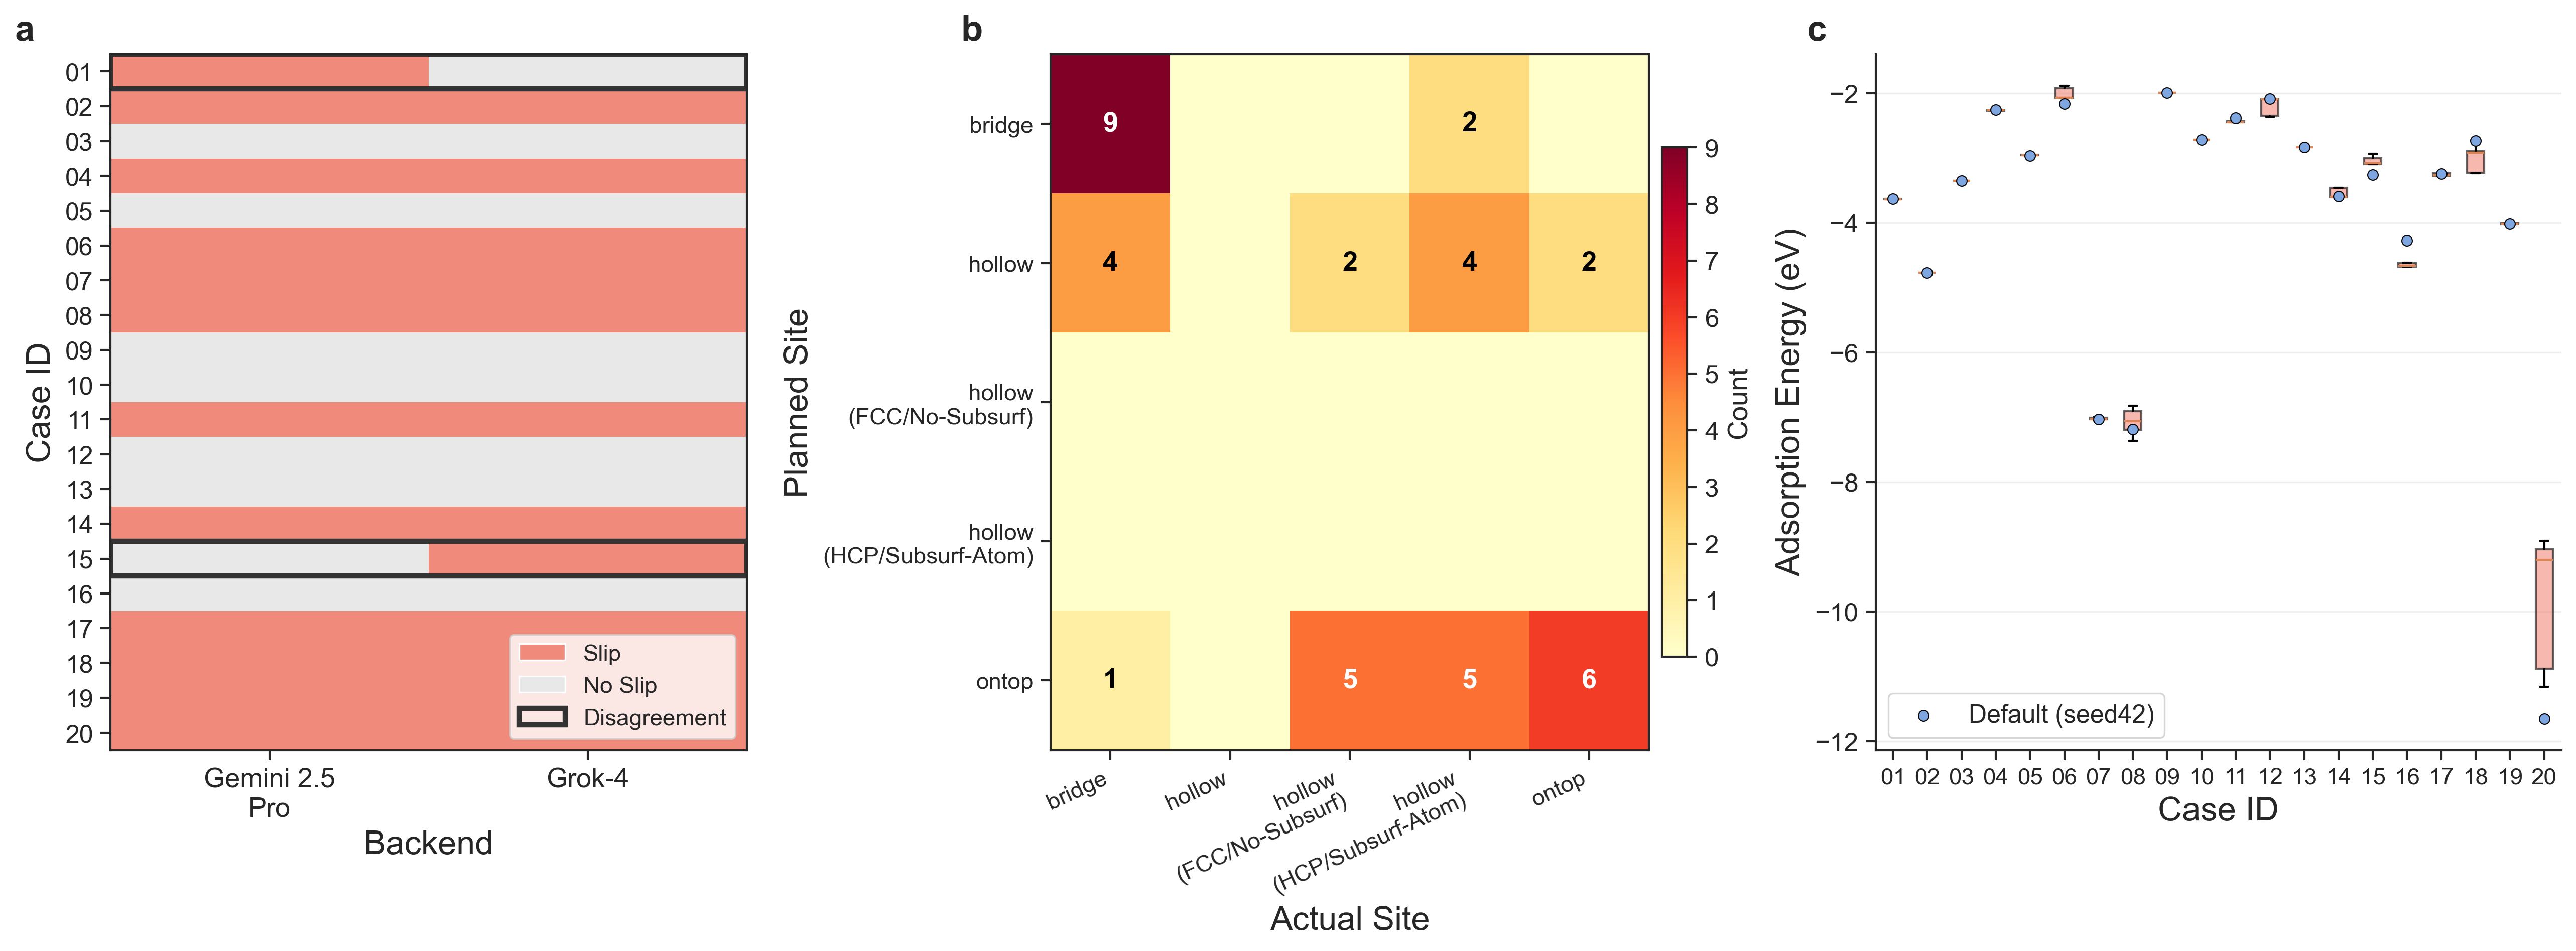
\includegraphics[width=\textwidth]{si_figures/si_figure_S2_combined.png}
    \caption{Supplementary Figure~S2: Slip and reproducibility. \textbf{(a)} Cross-backend slip agreement heatmap for gemini and grok-4 across 20 cases; disagreement cases~01 and~15 are outlined. \textbf{(b)} Site transition matrix counting planned--to--actual site changes. \textbf{(c)} Multi-seed reproducibility of GPT-5.4 Full: distribution of five independent seeds (43--47) with default seed~42 overlaid as scatter points.}
    \label{fig:si-s2}
\end{figure}

\bibliography{refs}

\end{document}
